\documentclass[12pt,a4paper]{article}
\usepackage[UTF8]{ctex}
\usepackage{amsmath,amssymb}
\usepackage{xcolor}
\usepackage{hyperref}
\usepackage{geometry}
\usepackage{graphicx}
\geometry{margin=2.5cm}

\title{Quantum If / 量子条件分支}
\author{QuoNic}
\date{}

\begin{document}
\maketitle

\begin{center}
\textbf{Language / 语言特性} | 难度：中级 | 预计时间：10 分钟
\end{center}

\tableofcontents
\newpage

\section{为什么需要？}

量子条件分支是基于测量结果的量子控制流。

\subsection{经典局限}
\begin{itemize}
  \item 经典条件分支无法处理量子态
  \item 量子测量会破坏量子态
\end{itemize}

\subsection{量子优势}
\begin{itemize}
  \item 量子条件分支可以根据测量结果执行不同操作
  \item 是量子算法中条件逻辑的基础
  \item 支持量子纠错中的伴随子测量
\end{itemize}

\subsection{实际应用}
\begin{itemize}
  \item 量子纠错
  \item 量子隐形传态
  \item 量子算法设计
\end{itemize}

\section{快速上手}

\begin{verbatim}
from quonic import qgate, qif, qshow
from quonic.gates import H, X

# 量子条件分支
qgate(H, 0)
qif(0, lambda: qgate(X, 1))
qshow()
\end{verbatim}

\textbf{预期输出}：
\begin{verbatim}
backend: native | shots: 1024
Result:
  |00>     512  ( 50.0%)
  |11>     512  ( 50.0%)
\end{verbatim}

\section{原理详解}

\subsection{电路图}

\begin{center}
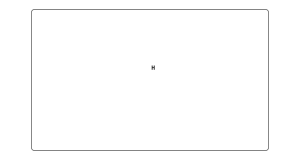
\includegraphics[width=0.6\textwidth]{../../images/qif_circuit.svg}
\end{center}

\subsection{数学推导}

量子条件分支：
\begin{equation}
|0\rangle|\psi\rangle \to |0\rangle|\psi\rangle \text{ or } |1\rangle X|\psi\rangle
\end{equation}

\textbf{测量后}：
\begin{itemize}
  \item 测量 $q_0 = 0$：不执行操作
  \item 测量 $q_0 = 1$：执行 $X$ 门
\end{itemize}

\subsection{几何解释}

量子条件分支在测量后根据结果执行不同操作。测量会塌缩量子态，然后根据经典结果执行量子门。

\section{代码详解}

\begin{verbatim}
from quonic import qgate, qif, qshow
from quonic.gates import H, X

# qif(qubit, true_fn, false_fn)
# qubit: 测量的量子比特
# true_fn: 测量为 1 时执行的函数
# false_fn: 测量为 0 时执行的函数
qgate(H, 0)
qif(0, lambda: qgate(X, 1))
qshow()
\end{verbatim}

\section{进阶用法}

\subsection{场景 1：量子纠错}

\begin{verbatim}
from quonic import qgate, qif
from quonic.gates import CX, X

# 量子纠错中的伴随子测量
qgate(CX, 0, 1)
qif(1, lambda: qgate(X, 2))  # 纠正错误
\end{verbatim}

\subsection{场景 2：量子隐形传态}

\begin{verbatim}
from quonic import qgate, qif
from quonic.gates import CX, H, X, Z

# 量子隐形传态
qgate(CX, 0, 1)
qgate(H, 0)
qif(0, lambda: qgate(Z, 2))  # 校正
qif(1, lambda: qgate(X, 2))  # 校正
\end{verbatim}

\section{适用场景}

\subsection{量子纠错}

量子条件分支用于量子纠错中的伴随子测量。根据测量结果执行纠正操作。

\subsection{量子隐形传态}

量子条件分支用于量子隐形传态中的校正操作。根据 Alice 的测量结果执行校正。

\section{常见问题}

\subsection{量子条件分支和经典条件分支有什么区别？}

量子条件分支基于量子测量结果，经典条件分支基于经典变量。量子测量会破坏量子态。

\subsection{量子条件分支会破坏量子态吗？}

是的，量子条件分支需要先测量量子态，测量会破坏量子态。

\section{学习路径}

\subsection{前置知识}
\begin{itemize}
  \item 量子测量
  \item 量子门
  \item 量子比特
\end{itemize}

\subsection{继续学习}
\begin{itemize}
  \item 量子纠错
  \item 量子隐形传态
  \item 量子算法设计
\end{itemize}

\section{完整示例代码}

\subsection{示例 1：基本量子条件分支}

\begin{verbatim}
from quonic import qgate, qif, qshow
from quonic.gates import H, X

qgate(H, 0)
qif(0, lambda: qgate(X, 1))
qshow()
\end{verbatim}

\section{下载}

\begin{itemize}
  \item [qif.py](https://github.com/ChrisLee0721/QuoNic/blob/main/examples/qif/qif.py)
\end{itemize}

\end{document}
